%%%%%%%%%%%%%%%%%%%%%%%%%%%%%%%%%%%%%%%%%%%%%%%
% latex_template_ieee_bbing.tex
%
% 28.02.2008  bsb Created 
%%%%%%%%%%%%%%%%%%%%%%%%%%%%%%%%%%%%%%%%%%%%%%%%%

% Final - 2 column style
%\documentclass[10pt,final,journal]{../latexlib/latex_ieee/IEEEtran}
% Draft - single column style
\documentclass[11pt,draftcls,journal,onecolumn]{../latexlib/latex_ieee/IEEEtran}

% If the IEEEtran.cls has not been installed into the LaTeX system files, 
% manually specify the path to it:
% \documentclass[conference]{../sty/IEEEtran} 

% Gives LaTeX2e the abilsity to do double column
%% correct bad hyphenation here
\hyphenation{op-tical net-works semi-conduc-tor IEEEtran}

% From thesis main (bbing)
\usepackage{amssymb,longtable,dcolumn}

% to use pdflatex
% Standard bbing packages
\usepackage{cite}      % Written by Donald Arseneau
\usepackage{graphicx}  % Written by David Carlisle and Sebastian Rahtz
\usepackage{url}       % Written by Donald Arseneau
\usepackage{amssymb,longtable,dcolumn}
\usepackage{bm}
%\usepackage{subfigure}
%\usepackage{stfloats}  % Written by Sigitas Tolusis
\usepackage[caption=false,font=footnotesize]{subfig}
%\usepackage{fixltx2e}
\usepackage{colortbl}
\usepackage{multirow}
\usepackage{amsmath}
\usepackage{units}
\usepackage{../latexlib/latex_cmds/math_bbing}
\usepackage{acronym}
\usepackage{csvsimple}
\usepackage{../latexlib/latex_cmds/my_acronyms}
\usepackage{color,soul}

\begin{document}

\newtheorem{remark}{Remark}
\renewcommand{\theremark}{\unskip}


\input{../latexlib/latex_cmds/Commands}  % shortcuts to thesis stuff
\input{../latexlib/latex_cmds/defs}
%\include{./latex_cmds/Commands}  % shortcuts to thesis stuff
%\include{./latex_cmds/defs}


% set the figure default size
\newcommand{\SF}{0.2}
\newcommand{\SFb}{0.45}
\newcommand{\SFPic}{0.45}
\newcommand{\SFPlot}{0.45}
\newcommand{\SFc}{0.25}
% Just a lazy way of setting the figure width (percentage of text width)
% 0.7 works well for 1 column
% 0.4 works well for 2 column
\newcommand{\FigWidth}{\SFb}

% Use this one for the draft version
\newcommand{\scaleOneTwo}[2] {\scalebox{#1}}
% Use this one for the two column version
%\newcommand{\scaleOneTwo}[2] {\scalebox{#2}}

% Graphics for this paper
\graphicspath{{images/}}

% paper title
%\title{Towards an Experimentally Validated Plume Model to Support Robotic Plume Characterization}
\title{Inertia Identification}

% author names and affiliations
% use a multiple column layout for up to three different
% affiliations
\author{Brian~Bingham$^{1}$% <-this % stops a space
\thanks{$^{1}$ Brian~Bingham is with the Department of Mechanical and Aerospace Engineering, Naval Postgraduate School, Monterey, CA 93950, USA. {\tt\small bbingham@nps.edu}}%
}

% make the title area
\maketitle

%\begin{abstract}
%Abstract
%\end{abstract}
% no keywords

\IEEEpeerreviewmaketitle

\section{Summary}
The general model we are using for surge and yaw is 
\[
m\dot{y}+k_1 y + k_2 y^2 = F
\]
where $y(t)$ is the forward speed or yaw rate, $m$ is the inertia, $k_1$ is the linear drag term, $k_2$ is the quadratic term, and $F$ is the constant thrust or torque.  If we assume $k_1 = 0$, so there is only quadratic drag, the solution to the differential equation takes the form
\[
y(t) = y_{ss} \tanh\left(y_{ss} \frac{k_1}{m} t \right)
\]
where $y_{ss}$ is the steady state velocity.  We know the drag coefficeint, $k_1$, from the steady-state experiment results, so there are two unknown parameters, the total inertia ($m$) and the steady-state velocity ($y_{ss}$).  

Experimentally we measured step response in surge and yaw.  The result is data for each step response experiment.  We can use MATLAB to fit a curve of the form above to the data, which results in something like...


\begin{figure}[htbp]
\centering
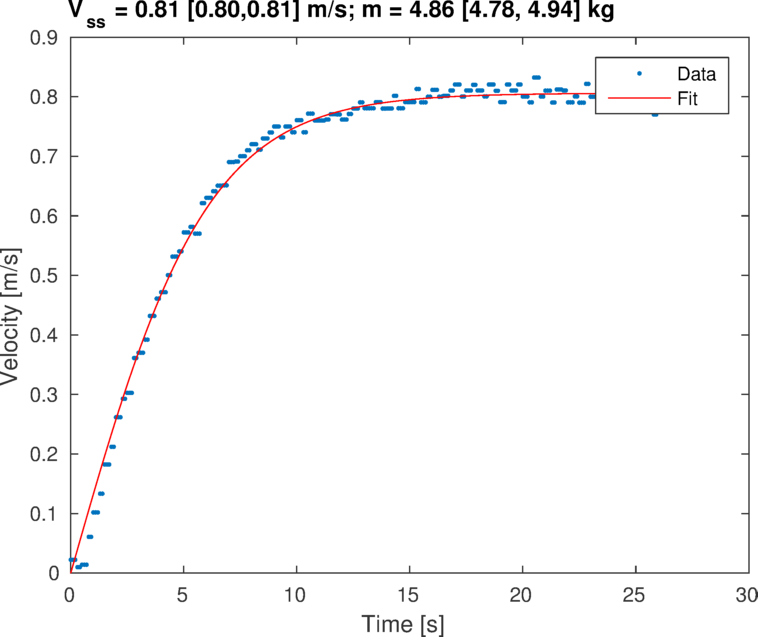
\includegraphics[width=0.9\linewidth]{fit_2.png}
\caption{Results from curve fit.  Parameter values are given as final value and 9\% confidence bounds.}
\label{f:t-cmd}
\end{figure}

\end{document}


